\chapter{Konzept, Entwurf und Implementierung}
\label{cha:implementierung}

% Abschnitt: Implementierungsdetails
\section{Implementierungsdetails}
\label{sec:implementierung:implementierungsdetails}

Wir erklären in diesem Kapitel die einzelnen Funktionen unserer Anwendung ausführlicher. Dies wird unterstützt durch Screenshots und den zugehörigen Mockups, die zu Beginn des Projekts erstellt wurden, um dem Kunden seine Vorstellungen visuell präsentieren zu können.\\

\begin{figure}[h]
    \centering
    \begin{minipage}{0.49\textwidth}
        \centering
        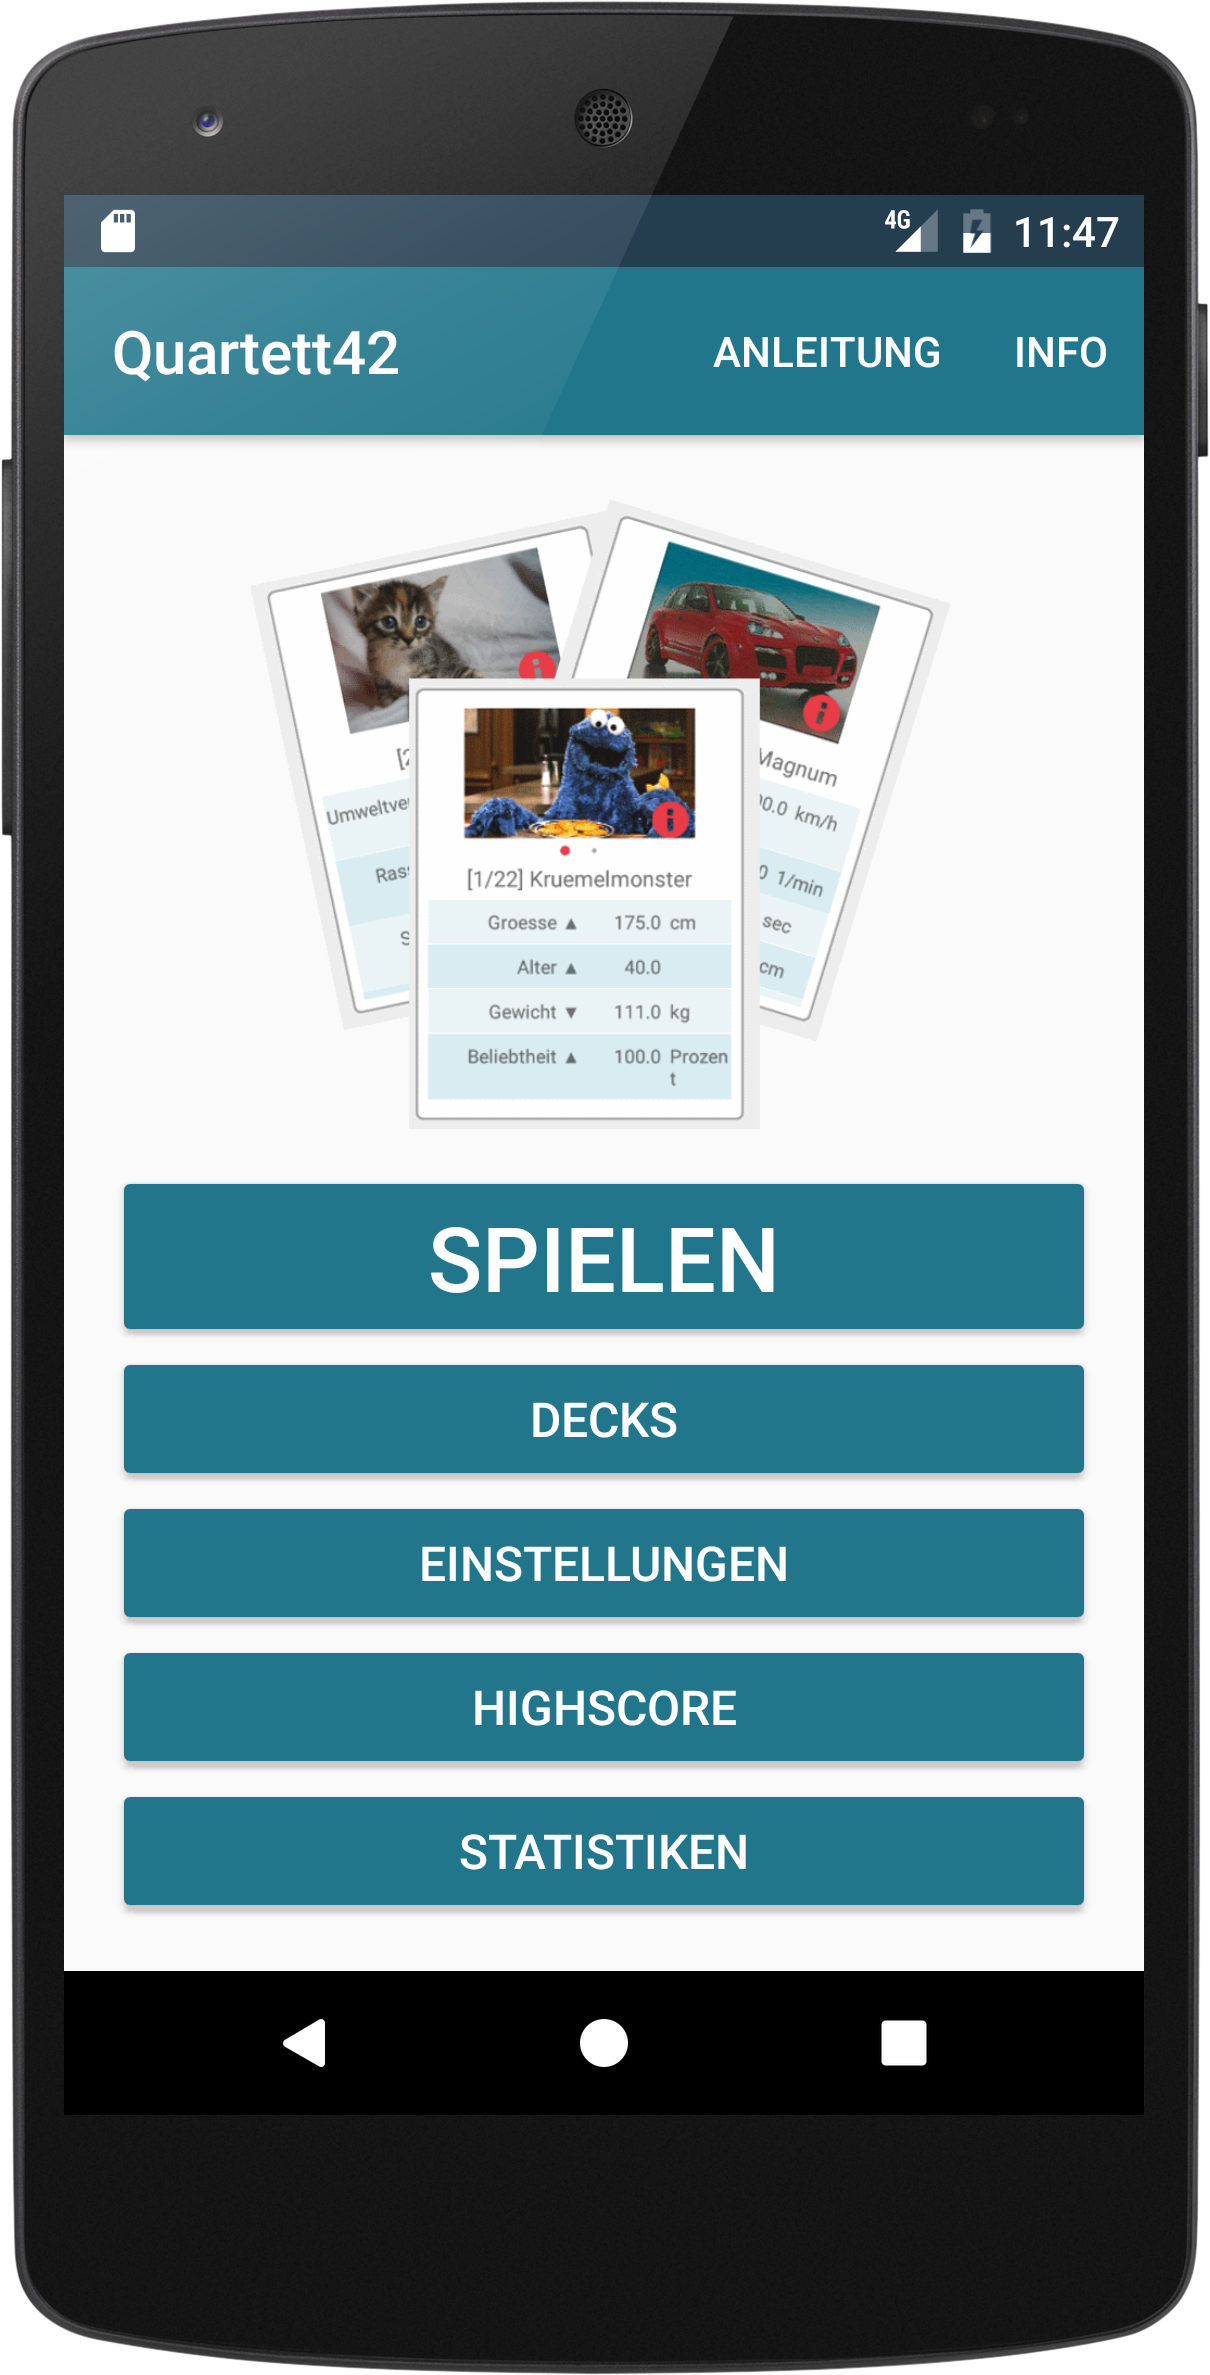
\includegraphics[width=0.4\textwidth]{img/screenshots/device_main_screen.png}
        \caption{Hauptmenü der App}
		\label{figure:implementierungmenue}
    \end{minipage}
    \begin{minipage}{0.49\textwidth}
        \centering
        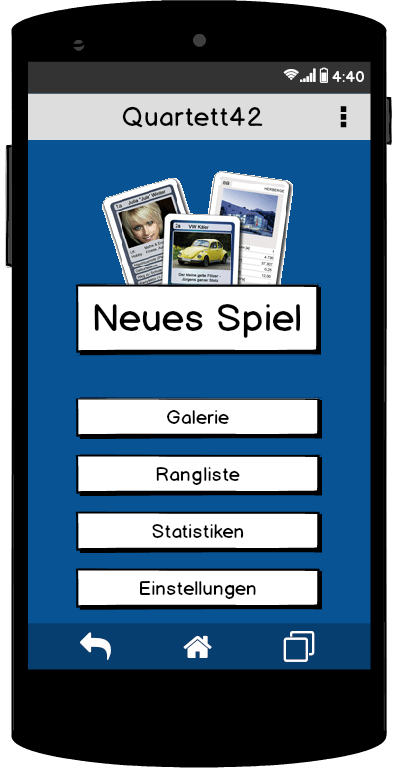
\includegraphics[width=0.4\textwidth]{img/mockups/main_screen.png}
        \caption{Mockup Hauptmenü}
    \end{minipage}
\end{figure}

Nach dem Öffnen der Anwendung befindet man sich zu Beginn im Hauptmenü, welches in Abbildung \ref{figure:implementierungmenue} zu sehen ist. Für das Hauptmenü, wie auch für die gesamte App, haben wir ein ansprechendes Farbklima gewählt. Wir entschieden uns für ein schlichtes und nicht zu verspieltes Design. Wir wollten eine App, deren Funktionen schnell ersichtlich sind und ohne Umstände bedient werden können. Außerdem wollten wir Bedienelemente wiederverwenden, die Benutzer bereits von anderen Android-Anwendungen kennen. Wir versuchten, das Design innerhalb der App konsistent zu halten und, wenn möglich, keine verschiedenen Elemente in verschiedenen Bereichen zu verwenden.

Durch den Menüpunkt 'SPIELEN' gelangt der Spieler auf einem Bildschirm, in welchem er ein Deck wählen kann und bei Bedarf die Einstellungen anpassen kann, wie in Abbildung \ref{figure:implementierungeinstellungen} zu sehen ist. Diese sind frei wählbar und alle Kombinationen sind möglich. Die Einstellungen werden lokal auf dem Smartphone gespeichert und können beim nächsten Start direkt benutzt werden, ohne sie jedes mal neu zu ändern. Das ermöglicht einen schnellen Start ins Spiel.\\

\begin{figure}[h]
    \centering
    \begin{minipage}{0.49\textwidth}
        \centering
        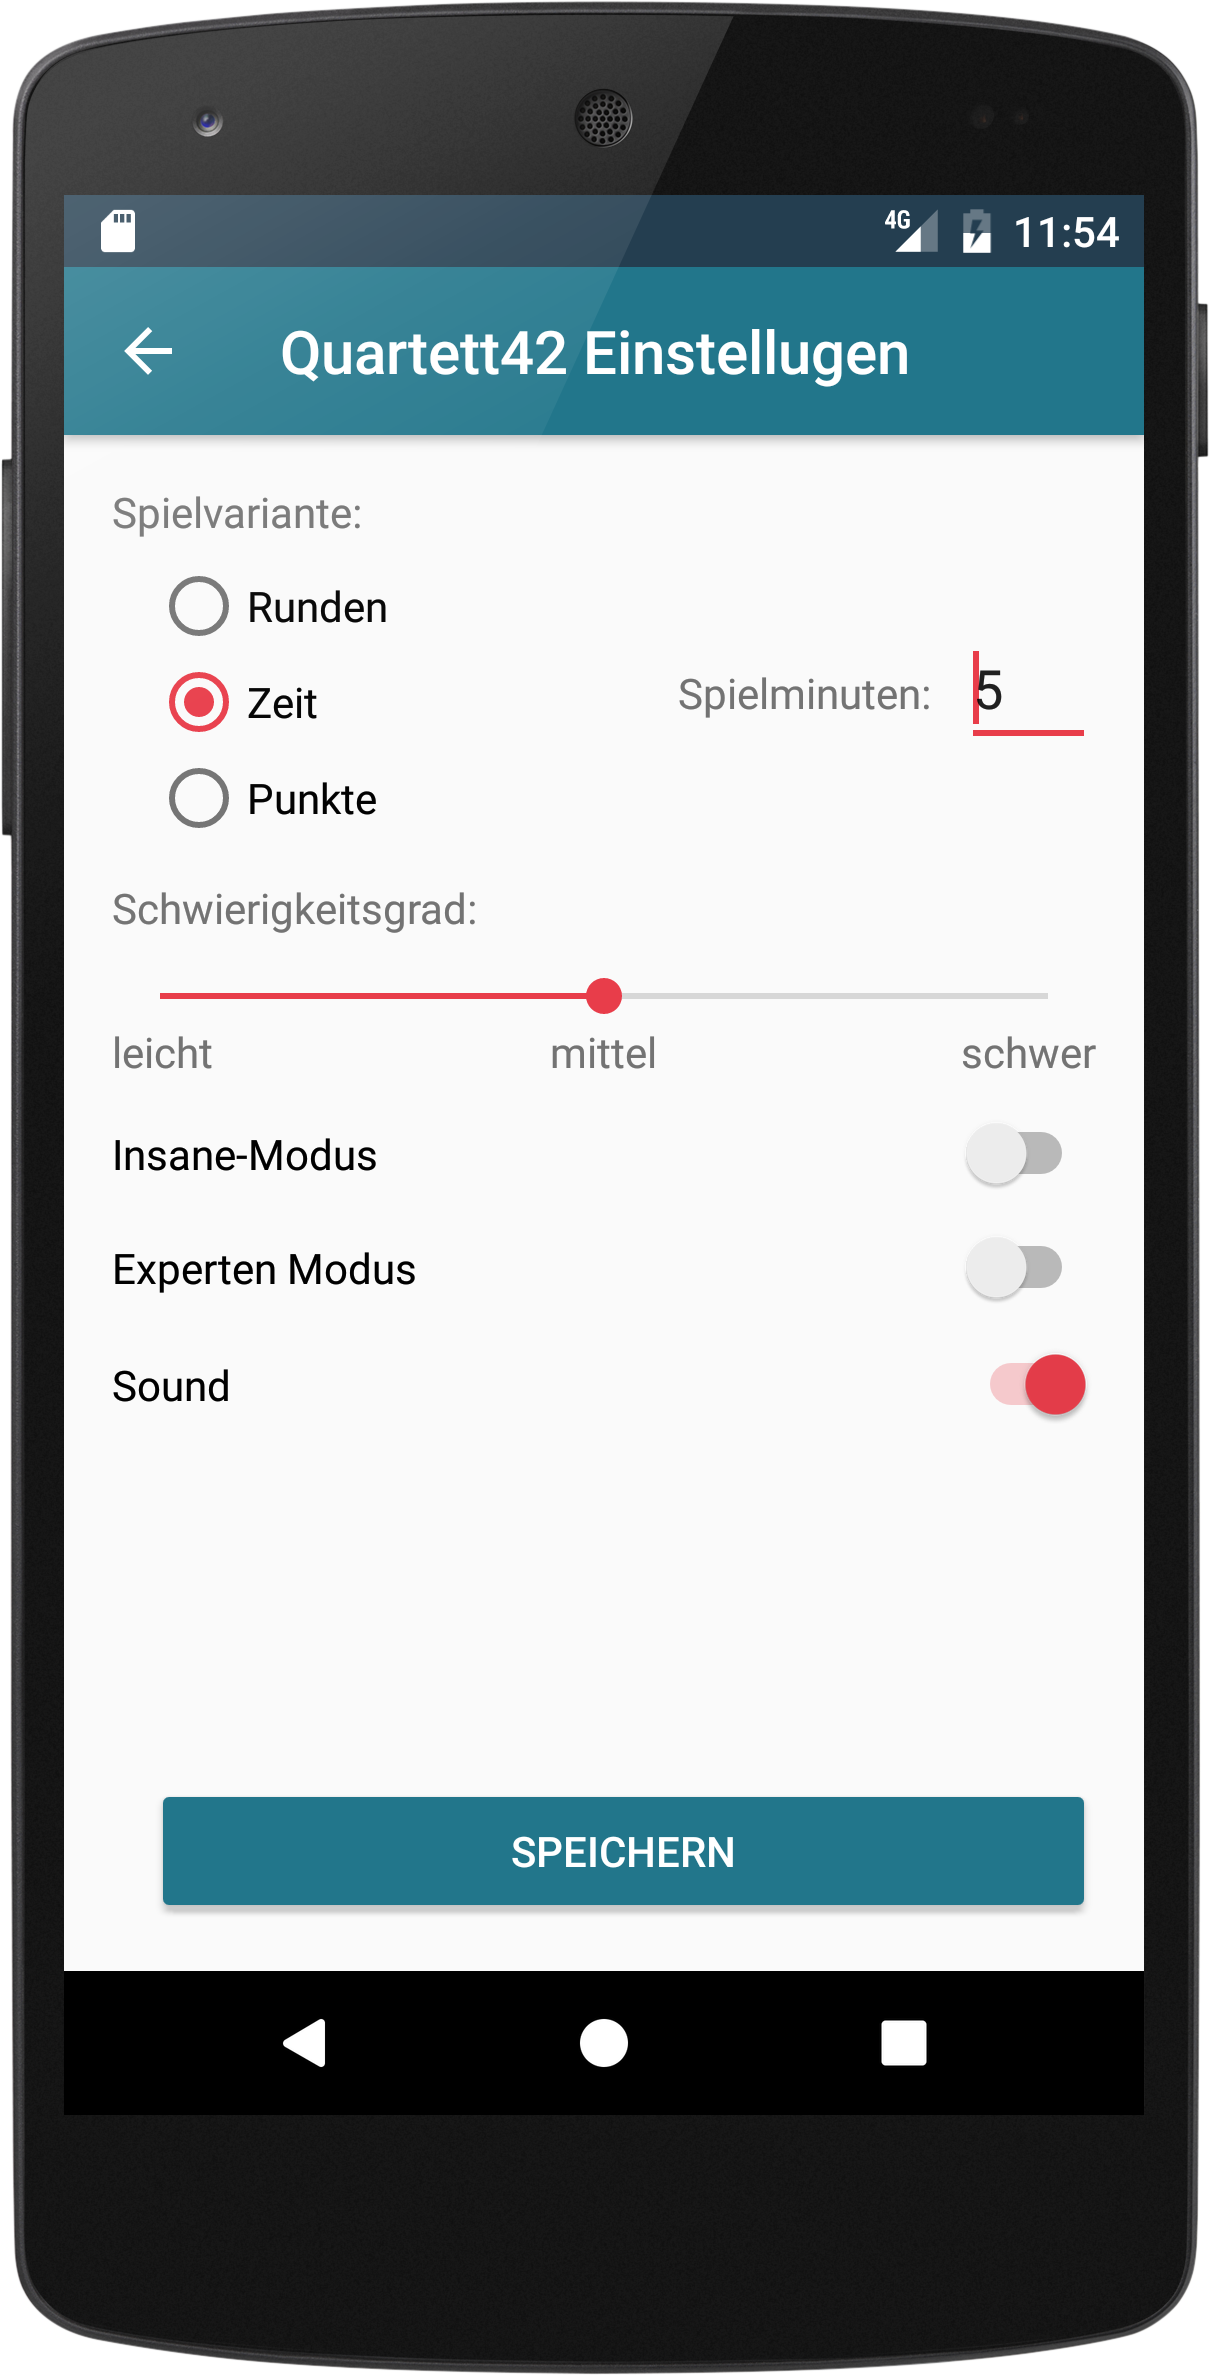
\includegraphics[width=0.4\textwidth]{img/screenshots/device_settings.png}
		\caption{Einstellungsmenü der App}
		\label{figure:implementierungeinstellungen}
    \end{minipage}
    \begin{minipage}{0.49\textwidth}
        \centering
        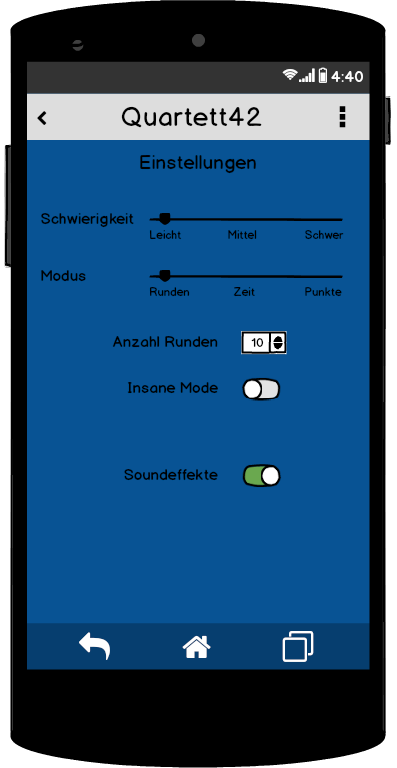
\includegraphics[width=0.4\textwidth]{img/mockups/einstellungen.png}
        \caption{Mockup Einstellungen}
    \end{minipage}
\end{figure}

Nun ist das eigentliche Spiel gestartet. Der Spieler sieht jeweils nur seine oberste Karte, wie in Abbildung \ref{figure:implementierungspiel1} zu sehen ist. Für jedes Attribut wird neben dem Wert (beziehungsweise einem Fragezeichen im ``Expertenmodus'') auch die jeweilige Einheit und die Siegesvariante (höher oder niedriger gewinnt) angegeben. Zwischen den Bildern einer Karte kann durch Swipe-Gesten gewechselt werden und zu jedem Bild kann, falls vorhanden, die passende Information durch drücken auf den Info-Button angezeigt werden. Wenn der Spieler am Zug ist, sind seine Attribute aktiv und er kann ein Attribut für den Vergleich auswählen. Für seinen Zug hat der Spieler unbegrenzt Zeit, außer im Zeitmodus, in welchem die Zeit für einen Zug auf 30 Sekunden beschränkt ist (die Zeit für seinen Zug wird dem Spieler angezeigt). Zudem werden die letzten 10 Sekunden durch ein akustisches Warnsignal begleitet, sofern in den Einstellungen die Sounds aktiviert sind. In allen Spielvarianten werden dem Spieler während des Spiels der aktuelle Zwischenstand (in Form von Punkten oder Karten) und die verbleibende Spielzeit (bzw. verbleibende Karten/Punkte) angezeigt.\\

\begin{figure}[h]
    \centering
    \begin{minipage}{0.49\textwidth}
        \centering
        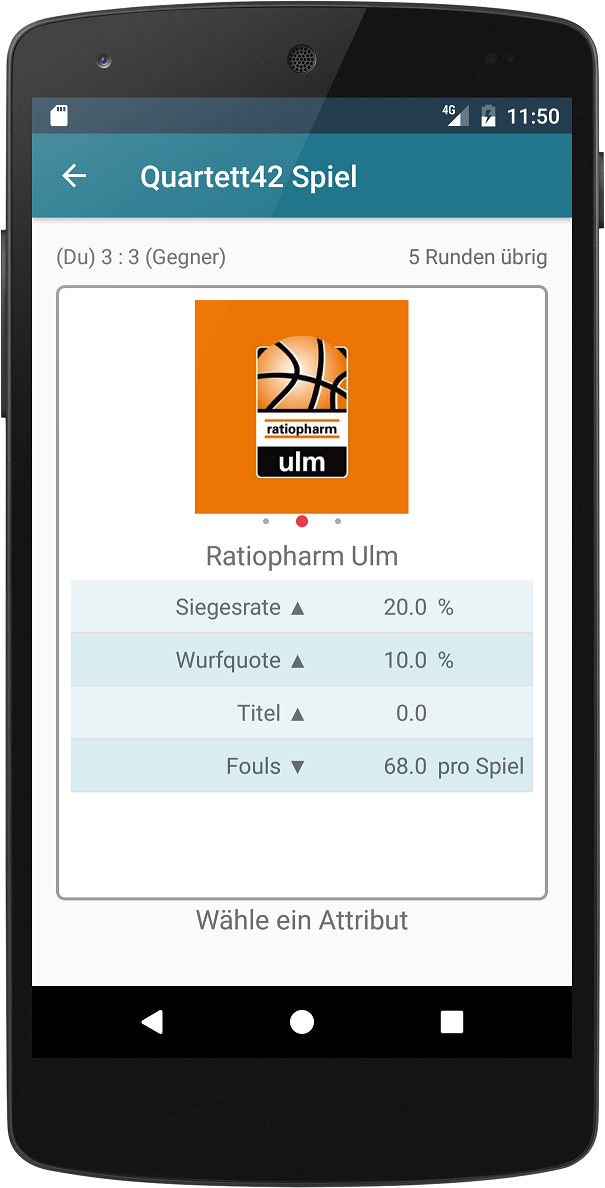
\includegraphics[width=0.4\textwidth]{img/screenshots/device_select_attr.png}
		\caption{Kartenansicht im Spiel}
		\label{figure:implementierungspiel1}
    \end{minipage}
    \begin{minipage}{0.49\textwidth}
        \centering
        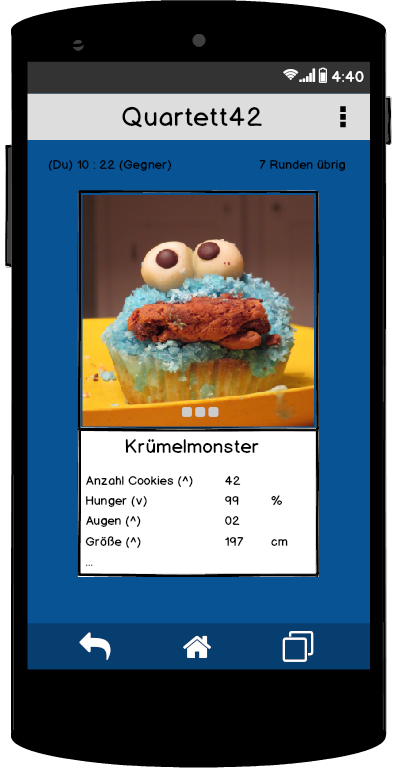
\includegraphics[width=0.4\textwidth]{img/mockups/spiel_attributauswahl.png}
        \caption{Mockup Karte im Spiel}
    \end{minipage}
\end{figure}


Ist der Gegner am Zug, sieht die Kartenansicht des Spielers gleich aus, aber seine Attribute sind inaktiv und nicht auswählbar. Nun muss der Spieler eine gewisse Zeit warten, bis der Computer sein Attribut für den Vergleich ausgewählt hat (es erscheint ein Text, der den Nutzer darauf hin weist). Diese Zeit kann er nutzen, um seine Karte zu betrachten. Im Schwierigkeitsgrad ``leicht'' wählt der Computer ein zufälliges Attribut für den Vergleich aus. Im Schwierigkeitsgrad ``mittel'' wählt er unter einer zufälligen Menge an Attributen, welche ungefähr die Mächtigkeit der Hälfte aller Attribute hat, den besten Wert aus. Im Schwierigkeitsgrad ``schwer'' wählt der Computer unter allen Attributen zu einer gewissen Wahrscheinlichkeit den besten Wert aus. Diese Schwierigkeitsgrade sorgen dafür, dass der Spieler zwar einen Anstieg der Schwierigkeit des Computers spürt, jedoch immer eine Chance zu gewinnen hat. Wir haben uns bemüht, den Zug des Computers so realistisch wie möglich zu gestalten. Deshalb hat der Algorithmus selbst bei der höchsten Schwierigkeitsstufe keine Informationen über die aktuelle Karte des Benutzers, es sind lediglich die Durchschnittswerte des Decks für jedes Attribut bekannt. Dies ist vergleichbar mit einem Spieler, der sehr oft mit einem Deck gespielt hat und ungefähr den durchschnittlichen Wert eines Attributs weiß. Zudem bliebt durch die Zufallswerte der Zug des Computergegners unvorhersehbar.

Nach jedem gespielten Zug sieht der Spieler den Vergleichsbildschirm mit seiner Karte und der Karte seines Gegners, wie in Abbildung \ref{figure:implementierungspiel2}  dargestellt (Wir sind hier insofern vom Mockup abgewichen, dass das Bild einer Karte mit dem gewählten Attribut angezeigt wird, statt nur alle Attribute anzuzeigen, da es so attraktiver aussieht). Dort kann wieder bei beiden Karten zwischen den Bildern durch Swipe-Bewegungen gewechselt werden und die jeweiligen Informationen durch Drücken des Info-Buttons angesehen werden. Der gewählte Wert beider Spieler wird angezeigt und der Gewinner hervorgehoben. Der Gewinner bekommt beide Karten, bei einem Unentschieden behält jeder Spieler seine Karte. Zudem wird der Punktestand aktualisiert. Im Kartenmodus und im Zeitmodus ist jede Karte genau ein Punkt wert. Im Punktemodus berechnen sich die Punkte für den Gewinner durch den prozentualen Unterschied beider Werte. So kann der Spieler mit ein und dem selben Attribut einer Karte unterschiedlich viele Punkte machen, je nachdem welche Karte der Gegner gerade besitzt. Außerdem ist es dadurch möglich, dass ein Spieler mit weniger Karten als der Gegner gewinnt, weil er durch geschickte Spielzüge mehr Punkte gesammelt hat.\\

\begin{figure}[h]
    \centering
    \begin{minipage}{0.49\textwidth}
        \centering
        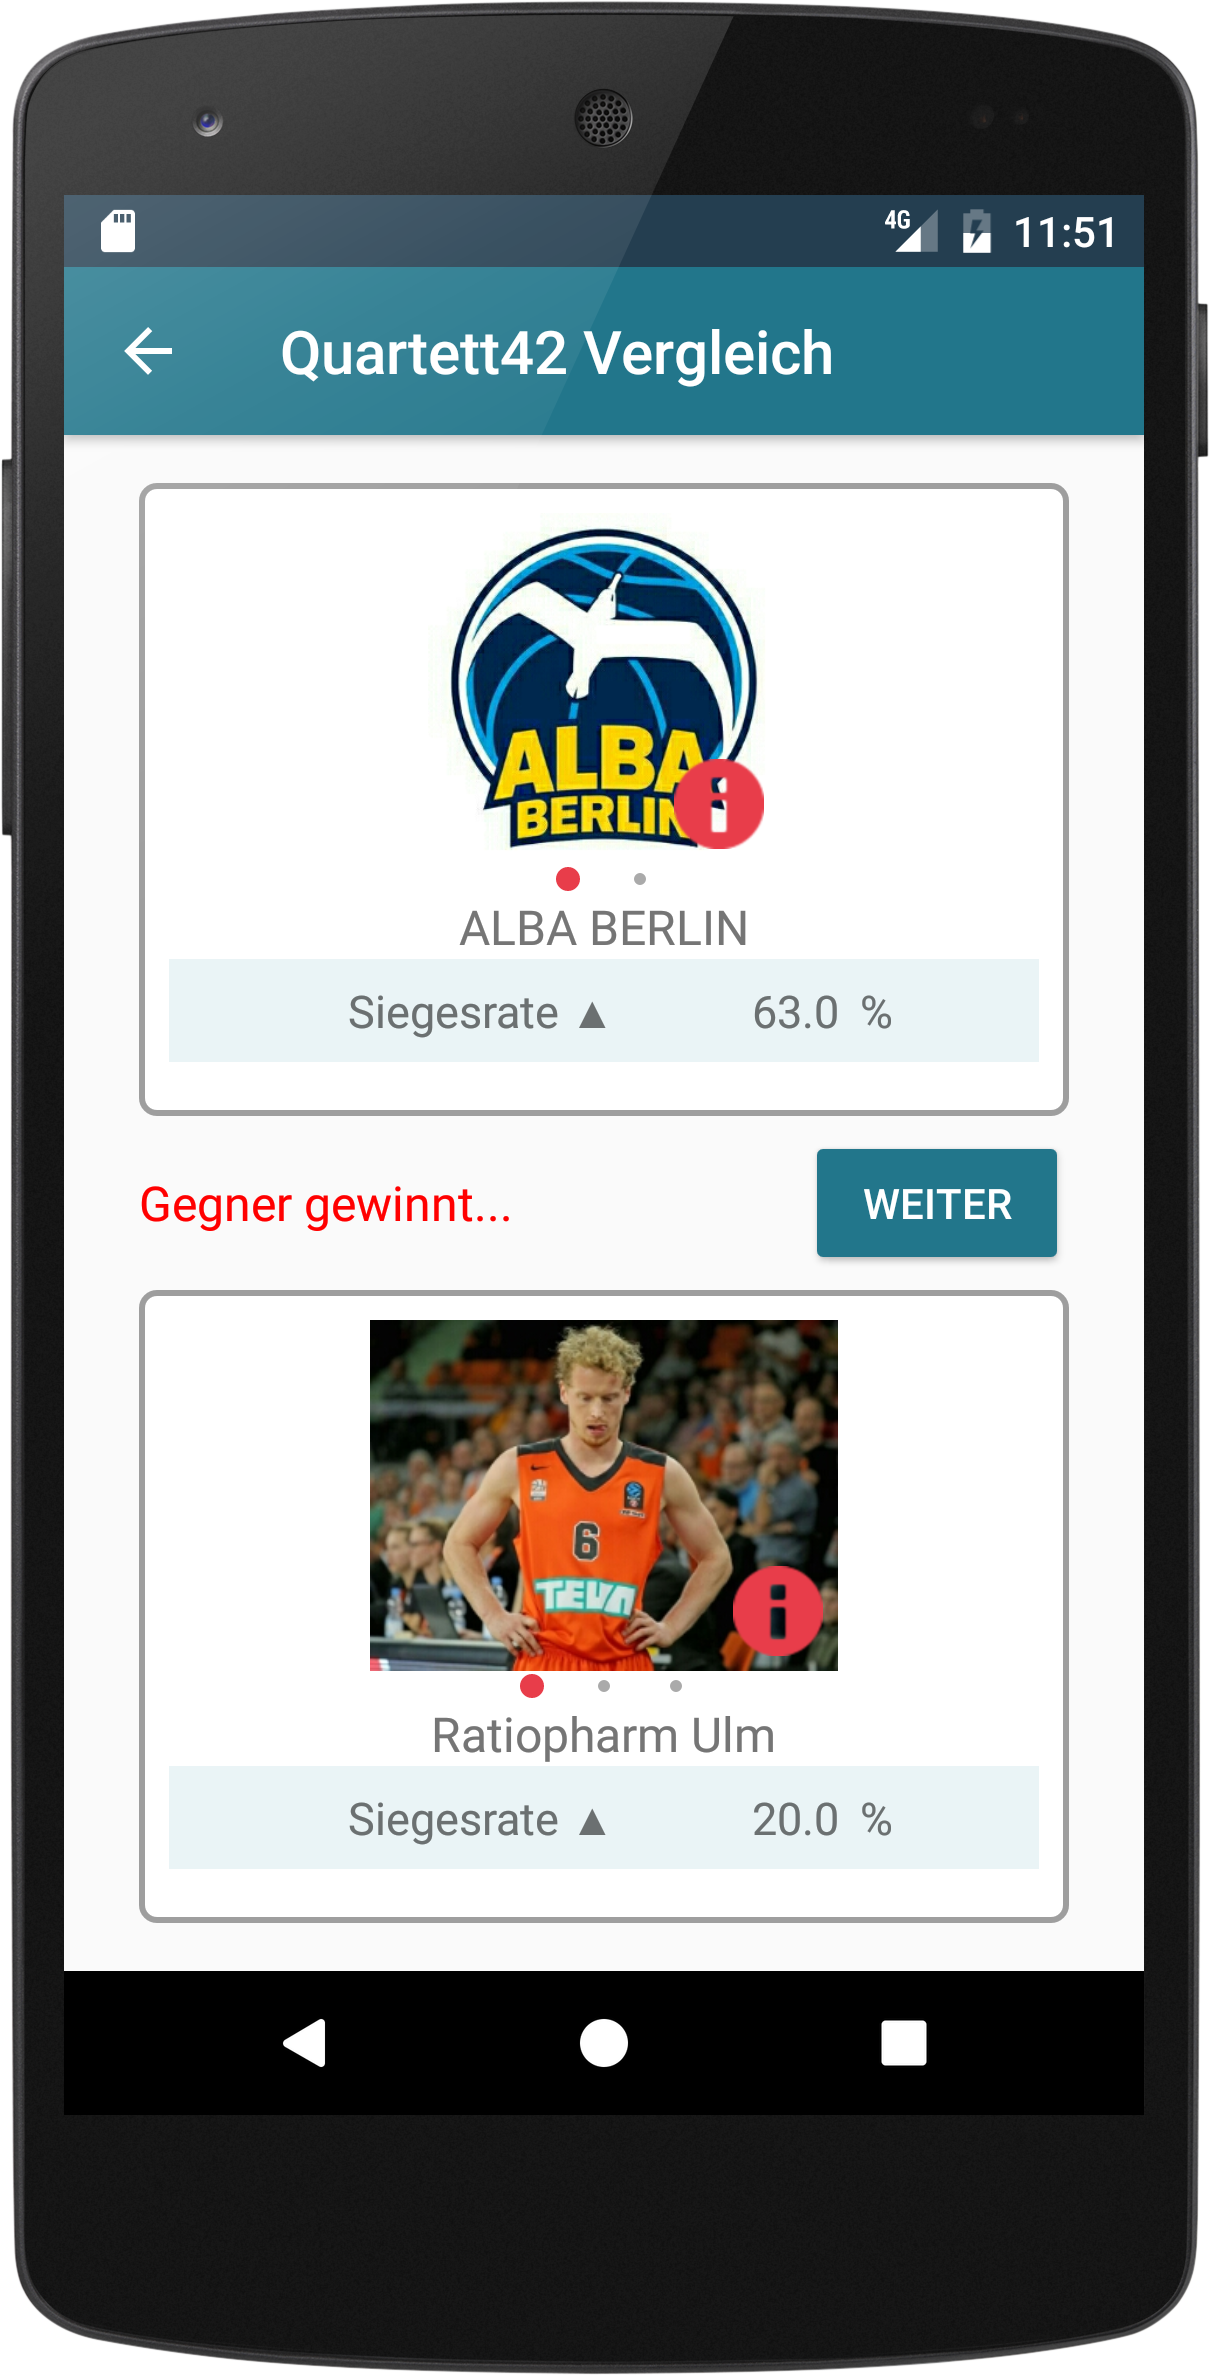
\includegraphics[width=0.4\textwidth]{img/screenshots/device_comparison.png}
		\caption{Kartenvergleich}
		\label{figure:implementierungspiel2}    
	\end{minipage}
    \begin{minipage}{0.49\textwidth}
        \centering
        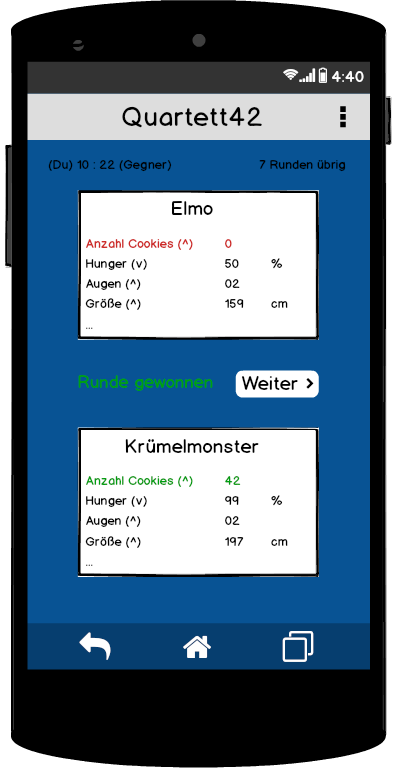
\includegraphics[width=0.4\textwidth]{img/mockups/spiel_vergleich.png}
        \caption{Mockup Kartenvergleich}
    \end{minipage}
\end{figure}


Der Spieler hat jederzeit die Möglichkeit, das laufende Spiel zu unterbrechen. Dazu wird ein Spiel automatisch zwischengespeichert, wenn der Spieler das laufende Spiel oder die App verlässt. Dieses kann der Spieler zu einem späteren Zeitpunkt fortsetzen. Wenn er ein neues Spiel beginnen möchte wird er gefragt, ob er lieber das alte Spiel fortsetzen will oder ein neues beginnen und das alte überschreiben möchte.

Steht ein Gewinner fest, wird der Spielend-Bildschirm angezeigt. Auf diesem steht der Gewinner, der Endstand und die gesammelten Punkte des Gewinners, wie in Abbildung \ref{figure:implementierungspielende} zu sehen.\\

\begin{figure}[h]
    \centering
    \begin{minipage}{0.49\textwidth}
        \centering
        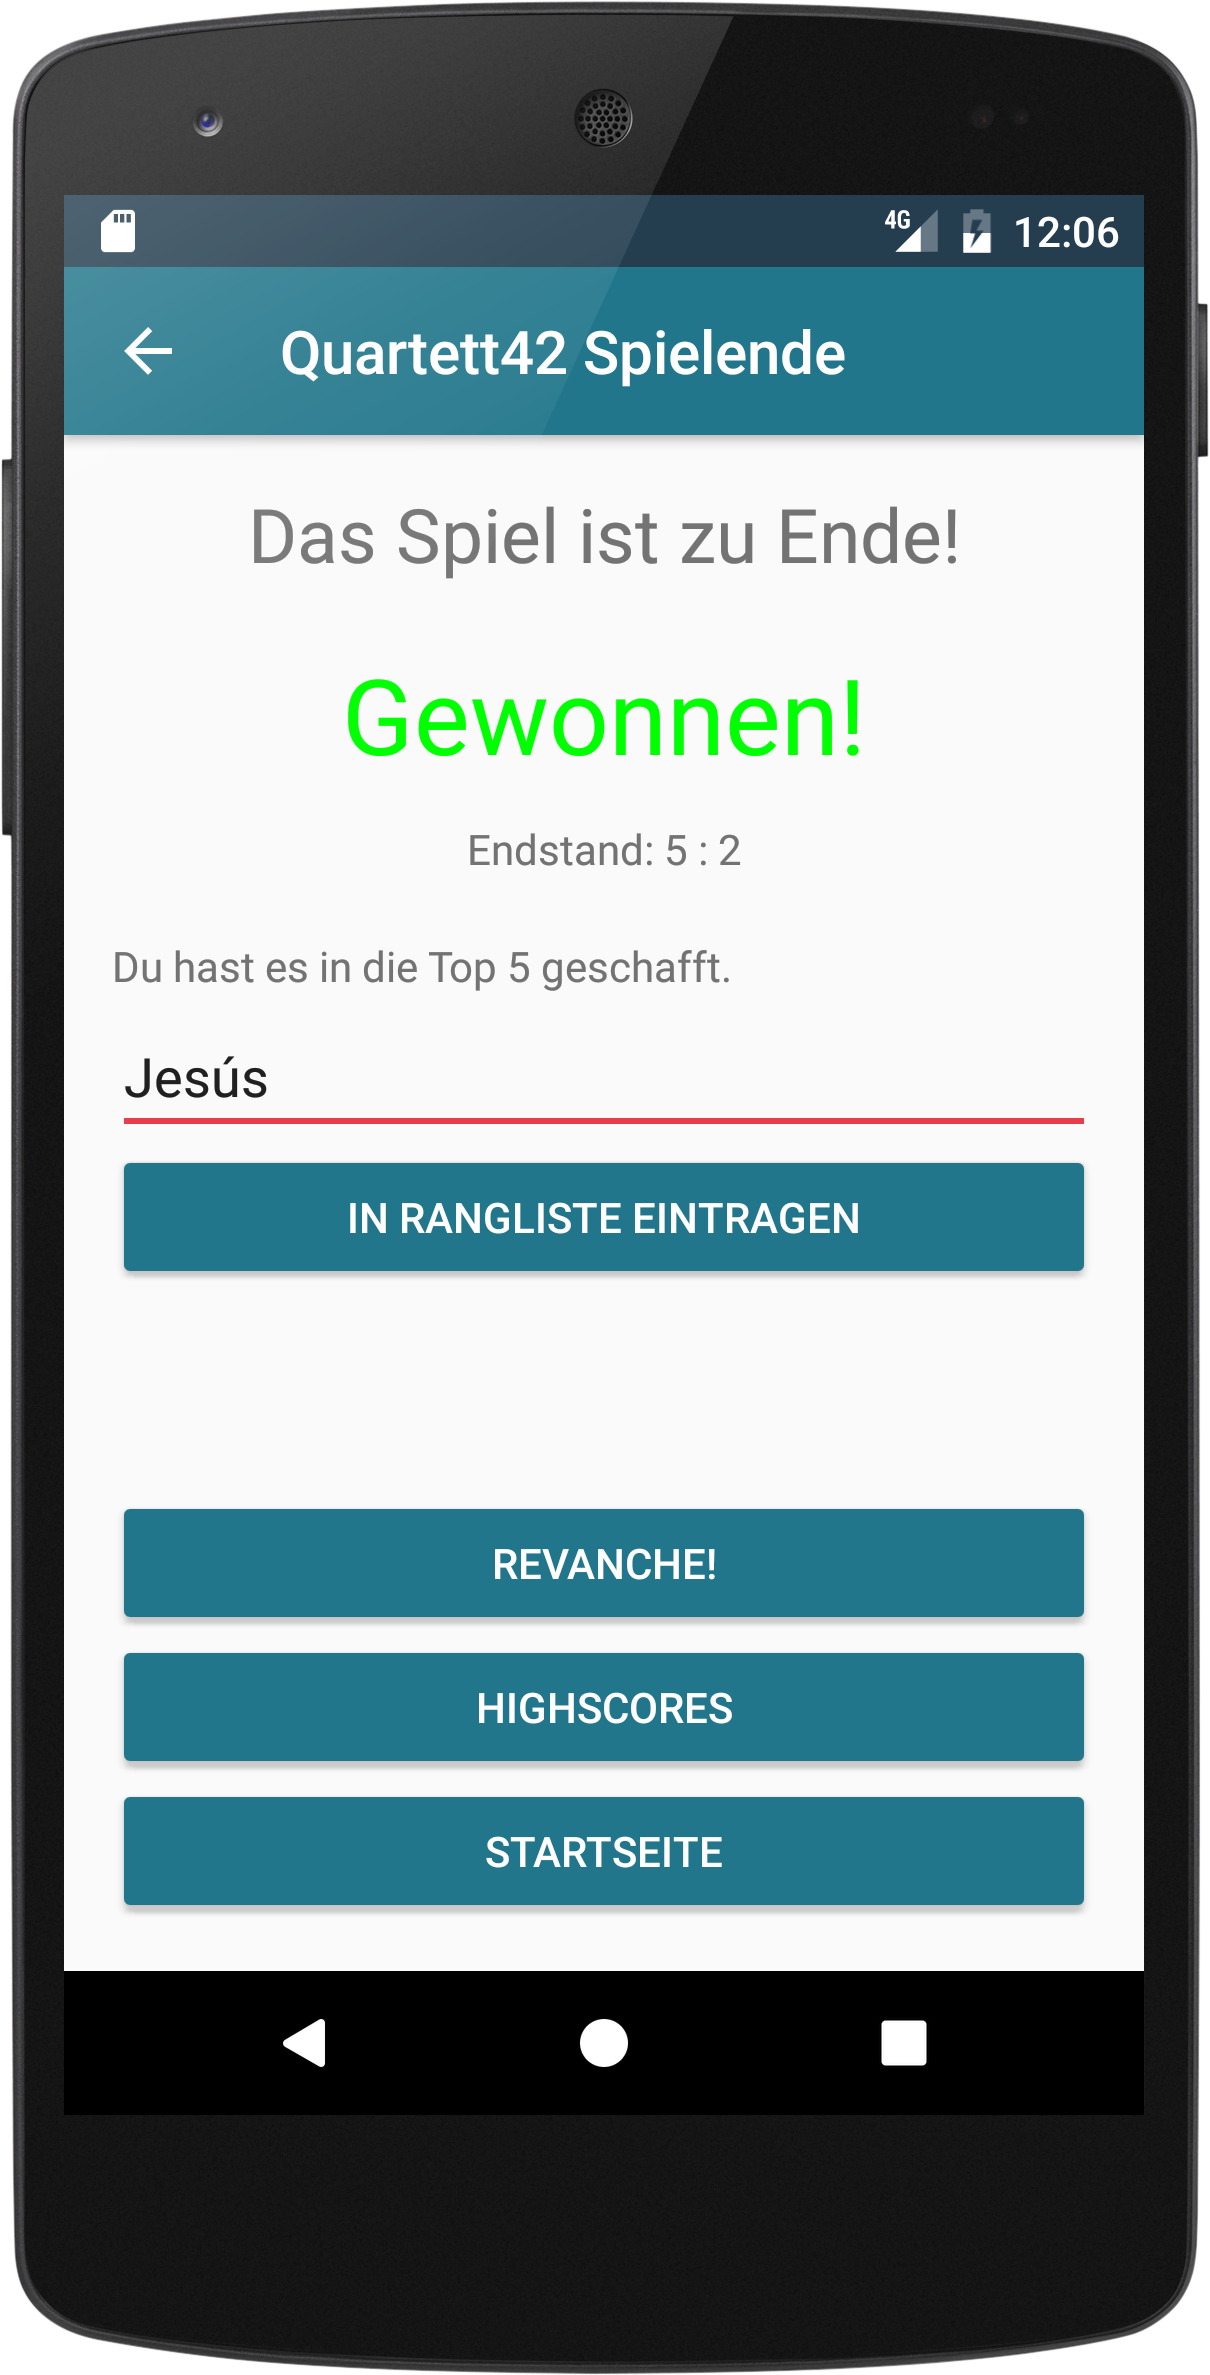
\includegraphics[width=0.4\textwidth]{img/screenshots/device_game_end.png}
		\caption{Endscreen der App}
		\label{figure:implementierungspielende}   
	\end{minipage}
    \begin{minipage}{0.49\textwidth}
        \centering
        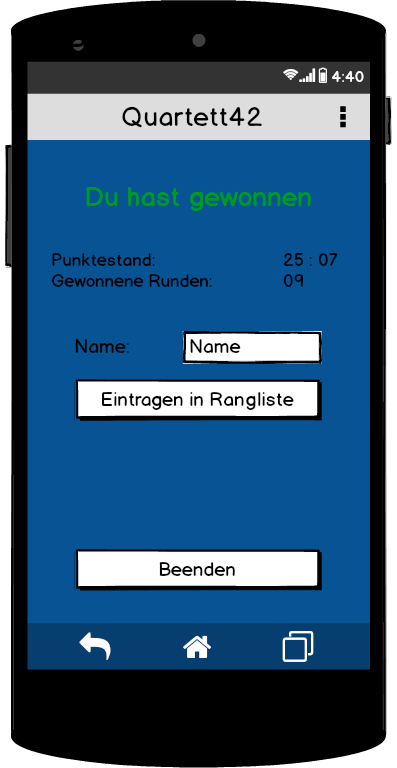
\includegraphics[width=0.4\textwidth]{img/mockups/spiel_ende.png}
        \caption{Mockup Endscreen}
    \end{minipage}
\end{figure}

Ist der Spieler der Gewinner, wird anhand dieser Punkte entschieden, ob der Spieler es in die Rangliste geschafft hat, und falls ja, auf welche Position. Die Punkte berechnen sich durch eine Kombination aus den gesammelten Punkten im Spiel, dem Schwierigkeitsgrad des Spiels, dem Spielmodus (normal, Insanemodus oder Expertenmodus) und der Anzahl der eingestellten Runden/Zeit/Punkte. Dadurch bleibt die Rangliste immer fair und kann nicht durch vereinfachte Einstellungen oder eine erhöhte Anzahl an Spielrunden beeinflusst werden. Der Spieler kann sich hier direkt mit seinem Namen in die Rangliste eintragen, wobei der jeweils letzte Name gespeichert wird. Außerdem kann er von diesem Bildschirm direkt die Ranglisten (Abbildung \ref{figure:implementierungrangliste}) einsehen oder eine Revanche starten, welche ein Spiel mit dem gleichen Deck und den gleichen Einstellungen startet.\\

\begin{figure}[h]
    \centering
    \begin{minipage}{0.49\textwidth}
        \centering
        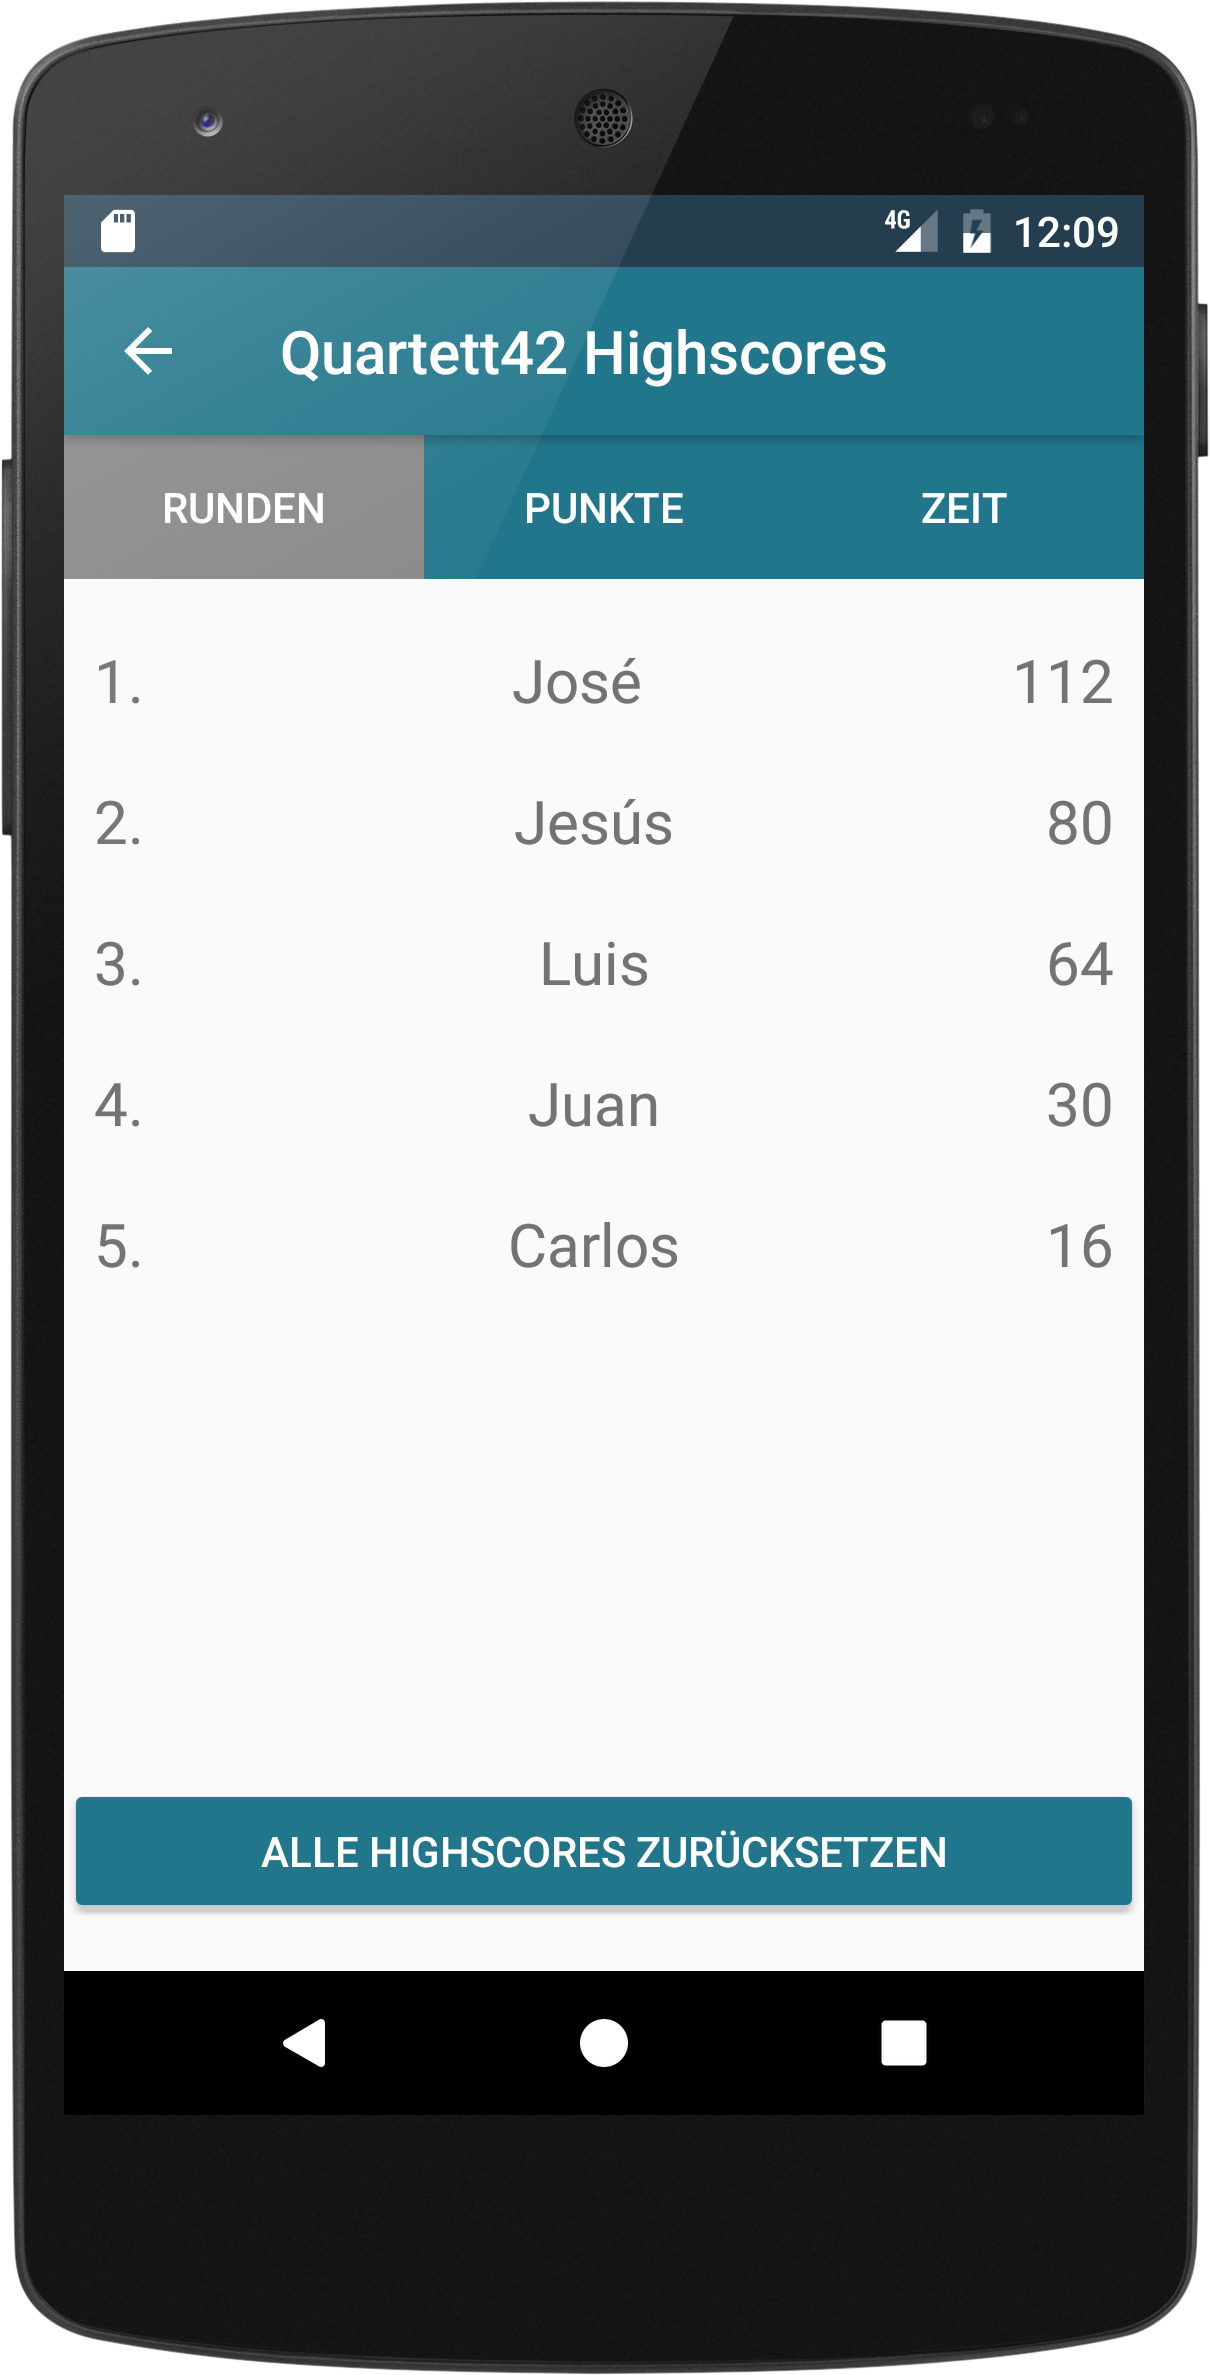
\includegraphics[width=0.4\textwidth]{img/screenshots/device_high_scores.png}
		\caption{Rangliste der App}
		\label{figure:implementierungrangliste}   
	\end{minipage}
    \begin{minipage}{0.49\textwidth}
        \centering
        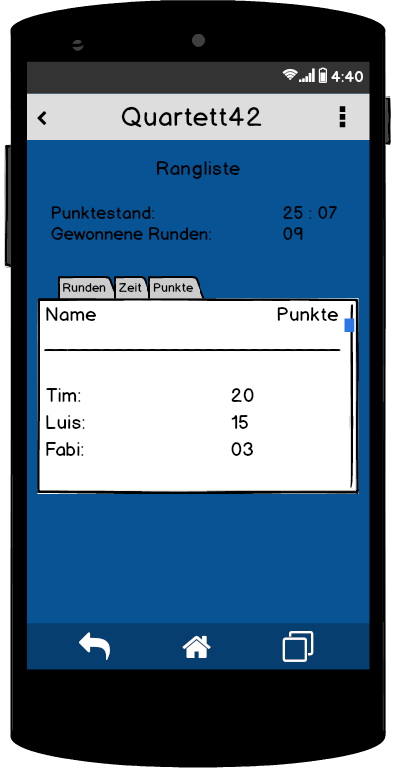
\includegraphics[width=0.4\textwidth]{img/mockups/rangliste.png}
        \caption{Mockup Rangliste}
    \end{minipage}
\end{figure}

Neben dem Spiel selbst befinden sich die meisten Implementierungsdetails unserer Anwendung im Menüpunkt 'GALERIE'. Dort hat der Spieler eine Übersicht aller Decks, die auf dem Smartphone vorhanden sind. Dieses Menü wurde durch ein Grid-Layout-Adapter erstellt und findet sich an vielen Stellen in unserer App wieder. Es erlaubt neben einer einfachen und immer gleich großen und gleich formartierten Darstellung der Bilder auch ein einfaches Scrollen und Anzeigen von Deckinformationen über den jeweiligen Info-Button. Ein Bild davon gibt es in Abbildung \ref{figure:implementierunggalerie}. 

\begin{figure}[h]
    \centering
    \begin{minipage}{0.49\textwidth}
        \centering
        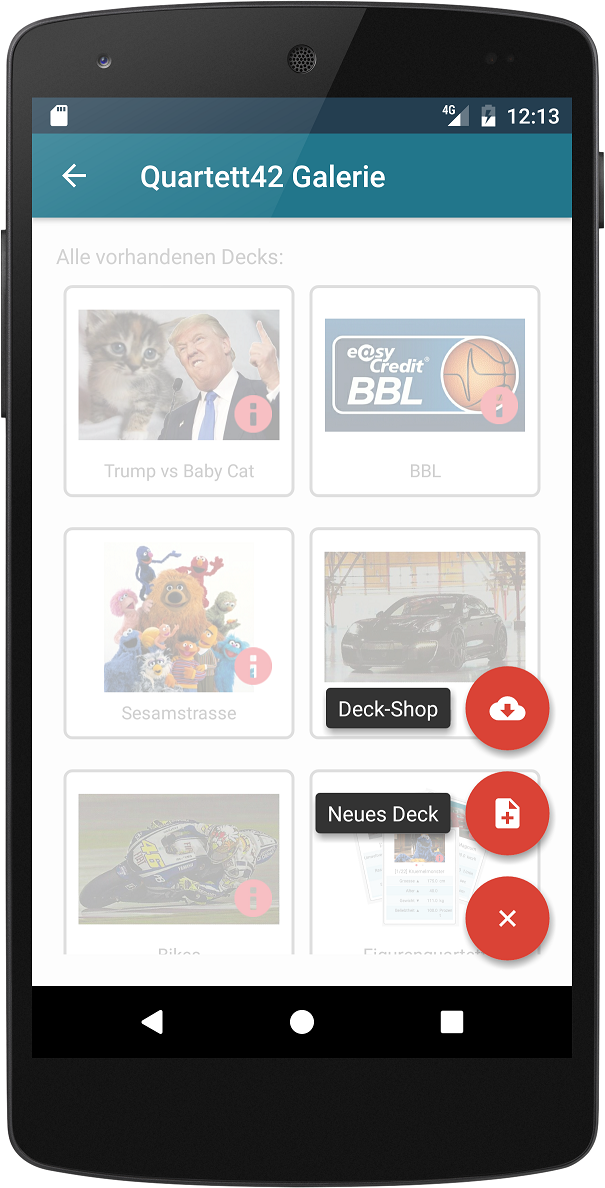
\includegraphics[width=0.4\textwidth]{img/screenshots/device_gallery.png}
		\caption{Die Galerie der App}
		\label{figure:implementierunggalerie} 
	\end{minipage}
    \begin{minipage}{0.49\textwidth}
        \centering
        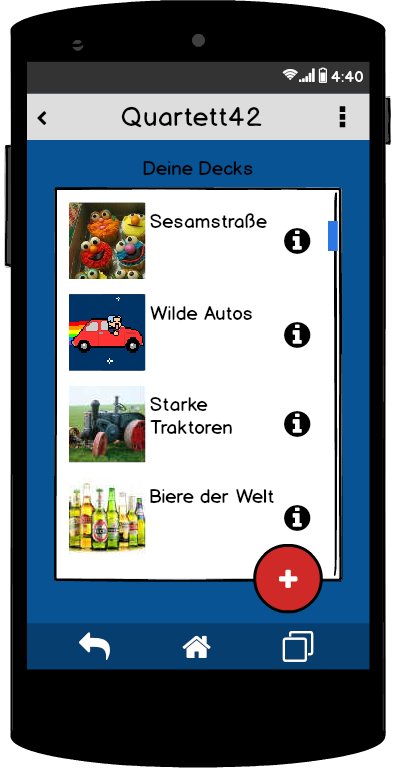
\includegraphics[width=0.4\textwidth]{img/mockups/galerie_uebersicht.png}
        \caption{Mockup Galerie}
    \end{minipage}
\end{figure}

Im Menü kann der Spieler die Karten eines Decks angucken, was ungefähr ähnlich ausieht wie die Kartenansicht während eines Spiels in Abbildung \ref{figure:implementierungspiel1}. Zudem kann er hier die Namen der Decks umbenennen, die einzelnen Werte und Bilder mit dazugehörigen Beschreibungen einzelner Karten der Decks ändern sowie neue Karten zu Decks hinzufügen oder Karten löschen. Außerdem kann ein Deck auch gelöscht werden oder über den Deckcreator ein völlig neues Deck mit neuen Attributen erstellt werden. Neue Decks können dann auf den Deckstore hochgeladen werden, sodass es für andere Nutzer zur Verfügung steht. Über diesen können wiederum auch neue Decks von anderen Nutzern auf das Smartphone herunter geladen werden. Auf diese zuletzt genannten Funktionen werden wir in den Besonderheiten genauer eingehen.\\

Neben der Rangliste gibt es auch noch einige Statistiken in unserer App, wie zum Beispiel die Anzahl der gespielten Spiele und die dabei gewonnen und verlorenen Spiele für die verschiedenen Spielmodi. Diese werden mit Hilfe der Bibliothek MPAndroidCharts als Piechart dargestellt und werden nach jedem bis zum Ende durchgespielten Spiel aktualisiert. Ein Bild davon gibt es in Abbildung \ref{figure:implementierungstatistiken}.\\

\begin{figure}[h]
    \centering
    \begin{minipage}{0.49\textwidth}
        \centering
        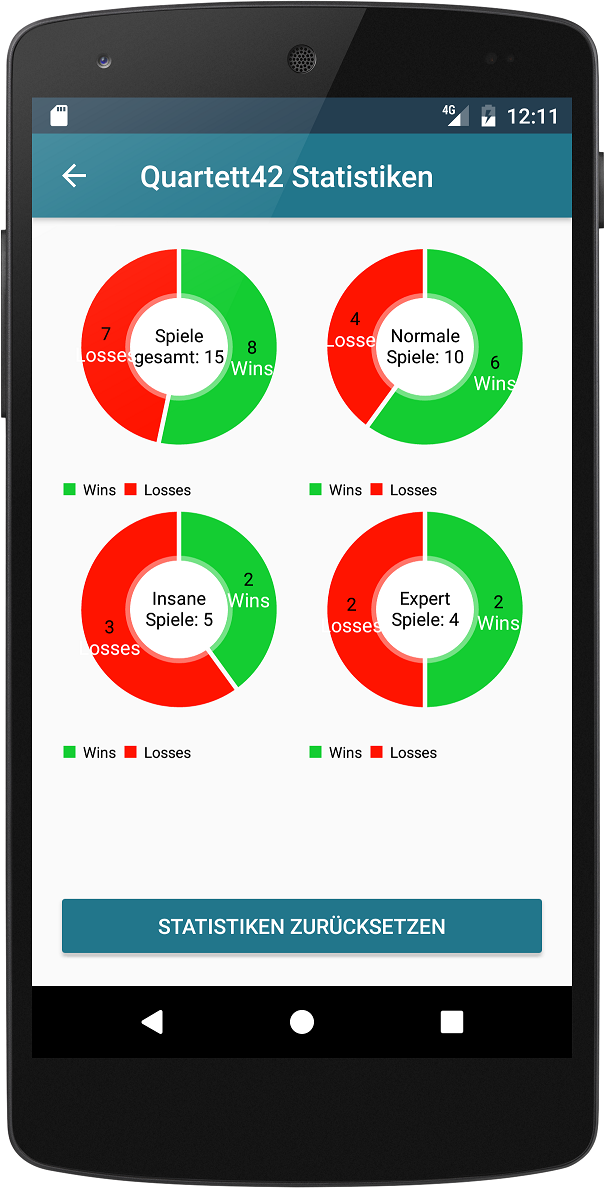
\includegraphics[width=0.4\textwidth]{img/screenshots/device_statistics.png}
		\caption{Die Statistiken der App}
		\label{figure:implementierungstatistiken}
	\end{minipage}
    \begin{minipage}{0.49\textwidth}
        \centering
        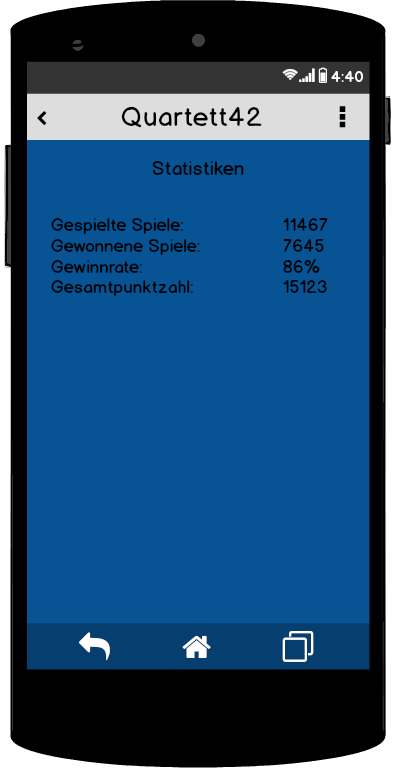
\includegraphics[width=0.4\textwidth]{img/mockups/statistiken.png}
        \caption{Mockup Statistiken}
    \end{minipage}
\end{figure}


% Abschnitt: Besonderheiten 
\section{Besonderheiten}
\label{sec:implementierung:besonderheiten }

Im Vergleich zu anderen Quartett-Apps gibt es bei unserer Quartett42-App neben den verschiedenen Spielmodi und Decks besonders zwei Funktionen, die so bisher noch nicht verfügbar waren. Diese sind zum einen unser Deckcreator und -editor und zum anderen der Deckstore mit Funktionen zum hoch- und herunterladen von Decks.	

\subsection{Deckcreator und -editor}
\label{sec:implementierung:besonderheiten:deckcreator }

\begin{figure}[htp]
	\centering
  	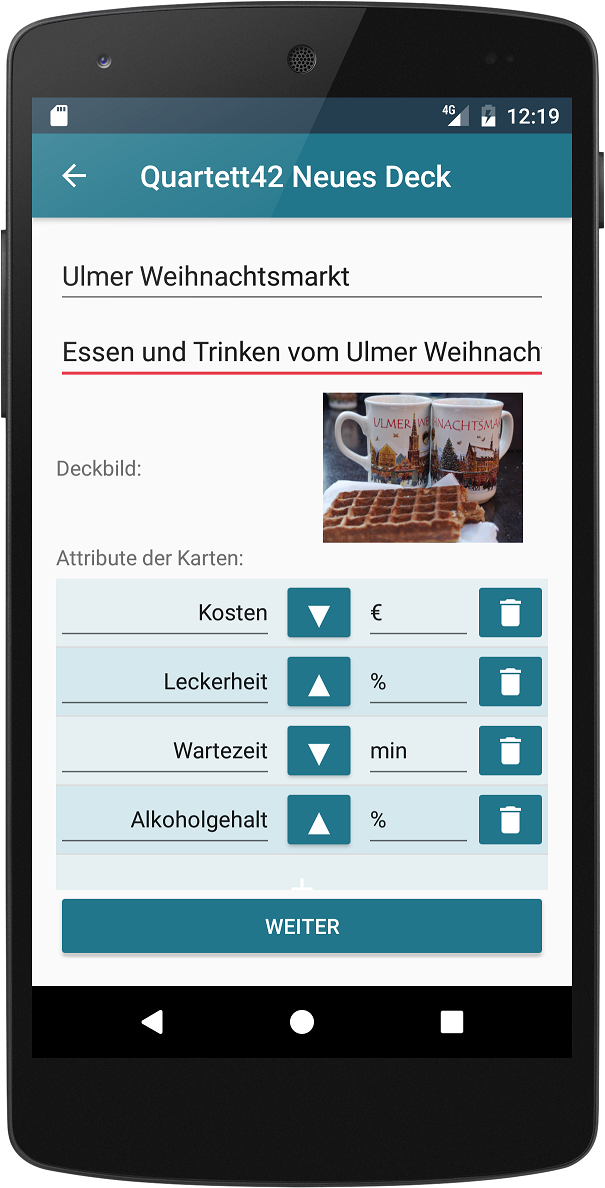
\includegraphics[width=0.3\textwidth]{img/screenshots/device_new_deck.png}
	\caption{Erster Schritt im Deckcreator}
	\label{figure:implementierungdeckcreator}
\end{figure}

Der Deckcreator erlaubt das Erstellen neuer Decks oder das Bearbeiten vorhandener Decks. Dadurch kann jeder Spieler ein komplett neues eigenes Deck nach seinen Wünschen erstellen. Über die Galerie gelangt der Spieler in den Deckcreator. Dort muss er erst einmal allgemeine Angaben zu seinem gewünschten Deck angeben, wie in Abbildung \ref{figure:implementierungdeckcreator} dargestellt. Dort muss ein Namen für das Deck eingegeben werden, wobei der Creator ein Deck nur erstellt, wenn dieser Name nicht bereits vergeben ist. Beschreibung und Bild sind optional, wobei bei keinem angegebenem Bild ein Standardbild verwendet wird. Das Bild kann entweder aus der Fotogalerie des Smartphones gewählt werden oder direkt aufgenommen werden, wobei es in beiden Fällen direkt auf eine akzeptable Größe verkleinert wird. Zudem müssen eine beliebige Anzahl an Attributen festgelegt werden, und für jede Attribut, wann es gewinnt, und welche Einheit es hat. Hier müssen verschiedene Überprüfungen statt finden. So darf kein Attribut zwei mal verwendet werden und es dürfen nirgends unerlaubte Zeichen oder leere Eingaben vorkommen. Sind alle Eingaben korrekt, wird das Deck zwischen gespeichert und der Nutzer zum zweiten Schritt weiter geleitet.

Im zweiten Schritt geht es um die Erstellung einzelner Karten und deren Werte. Wenn der Benutzer ein bereits vorhandenes Deck bearbeiten will, gelangt er direkt in diesen Schritt. Ein Bild davon kann man in Abbildung \ref{figure:implementierungdeckeditor} sehen.\\

\begin{figure}[htp]
	\centering
  	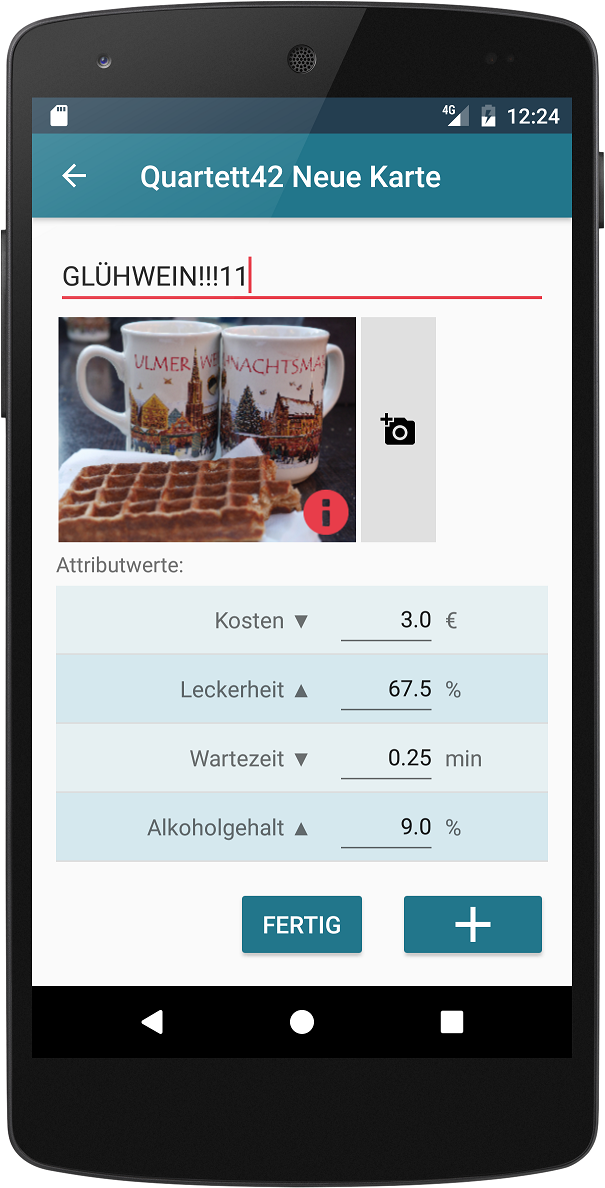
\includegraphics[width=0.3\textwidth]{img/screenshots/device_new_card.png}
	\caption{Zweiter Schritt im Deckcreator}
	\label{figure:implementierungdeckeditor}
\end{figure}

Für jede Karte muss ein Name eingegeben werden, welcher pro Deck wieder nur einmal vorkommen darf. Zudem kann eine beliebige Anzahl an Bildern wie beim Deckbild und dazu passende Beschreibungen angegeben werden. Für jedes Attribut der Karte muss ein Wert angegeben werden. Auch hierbei muss wieder alles auf gültige Eingaben überprüft werden und es dürfen keine leeren Eingaben vorkommen. Der Spieler kann jederzeit eine neue Karte hinzufügen und eine alte Karte löschen. Zudem kann er zwischen allen Karten hin und her wechseln. Dabei wird das Deck bei jedem Wechsel zwischengespeichert. Damit ein Deck spielbar ist, muss es mindestens zwei Karten besitzen. Ist der Nutzer fertig mit dem Erstellen oder Bearbeiten eines Decks, kann er es speichern und ansehen oder spielen. Zudem besteht die Möglichkeit, den Erstellvorgang zu unterbrechen und zu einer anderen Zeit fortzusetzen.

\subsection{Down- und Upload von Decks}
\label{sec:implementierung:besonderheiten:deckdownload }

Über den Deckstore können Decks hoch- und heruntergeladen werden. Das ermöglicht das Teilen von selbst erstellten Decks mit anderen und führt dazu, dass immer wieder neue Decks heruntergeladen werden können. Die Speicherung der Decks findet auf einem Server des Institutes für Datenbanken und Informationssysteme der Universität Ulm statt. Die Daten der Decks werden dabei als JSON-Strings gespeichert (dieser Dienst war nicht Teil unserer Implementierung).

Über die Galerie gelangt man in den Deckstore, in welchem dem Spieler alle Decks aus dem Deckstore angezeigt werden, welche er noch nicht selbst auf sein Smartphone herunter geladen hat. Diese erfragt die Anwendung durch einen HTTP-Request an den Server, welcher eine Liste alle auf dem Server vorhandenen Decks zurück liefert. Zudem wird für jedes Deck noch das Deckbild und die Deckbeschreibung heruntergeladen und zwischengespeichert. Außerdem erhält der Nutzer beim Starten der App eine Benachrichtigung in der Statusleiste, falls neue Decks im Deckstore verfügbar sind. Die Darstellung im Deckstore erfolgt wieder über den Grid-View-Adapter, ähnlich zu Abbildung \ref{figure:implementierunggalerie}. Der Benutzer kann nun ein Deck auswählen, welches er herunterladen möchte. Der Nutzer sieht während dem gesamten Ladevorgang einen Fortschrittsbalken, welcher den Fortschritt in Prozent berechnet und darstellt. Für das Deck wird dann zuerst die allgemeine Deckinformation heruntergeladen sowie eine Liste aller Karten. Dann wird jede einzelne Karte heruntergeladen und für jede Karte alle dazugehörigen Bilder und Werte. Für jede dieser Daten wird ein HTTP-Request an den Server gesendet, welcher die Daten in Form eines JSON-Strings zurück gibt. Da nicht nur unsere Anwendung, sondern mehrere Anwendungen Decks auf den Server hochladen können, welche nicht unbedingt formal korrekt sein können, wird in jedem Schritt überprüft, ob das Deck alle Anforderungen erfüllt. Dazu gehören zum Beispiel eine Mindestanzahl an Karten und Attributen, keine unerlaubten Zeichen und leere Angaben sowie keine fehlerhaften Bilddateien. Letztere werden durch ein Standardbild ersetzt, bei allen anderen Fehlern wird der Download abgebrochen, um unnötige Wartezeiten zu vermeiden. Bilder, die zu groß sind, werden automatisch verkleinert. Nach dem vollständigen Download aller Daten und der Kontrolle wird das Deck zusammen gebaut und in den lokalen Speicher gespeichert. Hierbei wird bevorzugt versucht, die Daten auf einem externen Speicher zu speichern, um nicht den internen Speicher zu belasten. Eine Grafik, wie der Download funktioniert, sieht man in Abbildung \ref{figure:implementierungdownundupload}.

In der Galerie hat der Benutzer die Möglichkeit, ein Deck direkt auf den Server hochzuladen. Zuerst wird durch eine Anfrage an den Server überprüft, ob das Deck schon im Deckstore vorhanden ist. Ist dies der Fall, kann das selbe Deck nicht erneut hochgeladen werden. Fall nicht, bekommt der Benutzer wieder eine Ladeanzeige mit Fortschrittsbalken zu sehen. Bevor das Deck hochgeladen wird, wird auch dieses zur Sicherheit auf Fehler überprüft, welche aber im Normalfall dank der Fehlerüberprüfung bei der Deckerstellung nicht vorkommen dürfen. Dann wird das Deck in viele einzelne JSON-Strings zerlegt und dem Server über einen HTTP-Request das Deck mit seinen Informationen bekannt gegeben. Danach wird wie beim Download, jede Karte und mit ihm seine Werte Werte und Bilder als JSON-String über einen extra HTTP-Request gesendet, wobei die Bilder in einen Base64-String konvertiert und versendet werden. Nach erfolgtem Upload ist das Deck für alle Benutzer über den Deckstore verfügbar. Abbildung \ref{figure:implementierungdownundupload} zeigt den Kommunikationsfluss beim Upload-Prozess. Sollte der Benutzer keine Internetverbindung haben, wird sowohl der Download als auch der Upload abgebrochen.
\newpage

%Download- und Upload-Verlauf-Modell
\begin{figure}[htp]
\centering
\begin{minipage}{.45\textwidth}
  \centering
  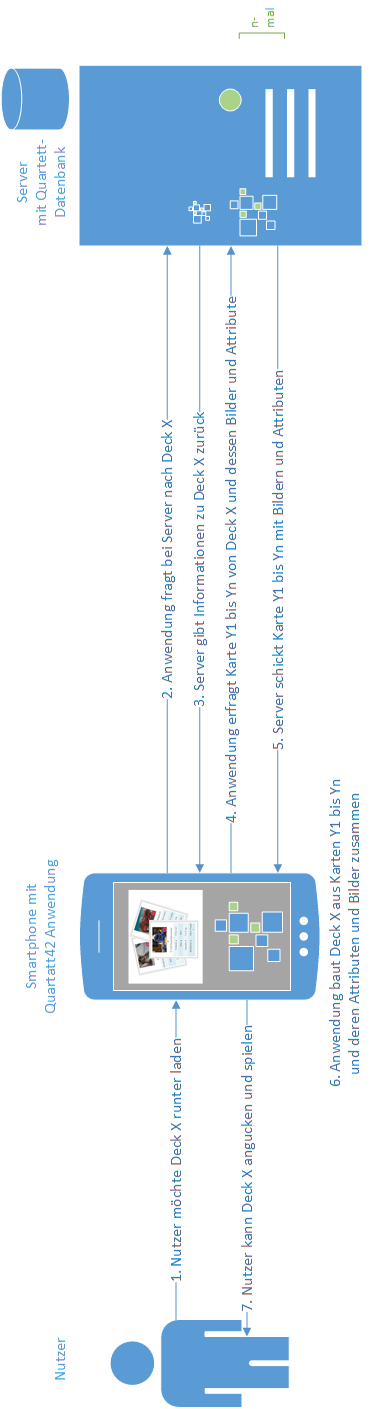
\includegraphics[width=.95\linewidth]{img/modelle/downloadmodell.png}
\end{minipage}%
\begin{minipage}{.45\textwidth}
  \centering
  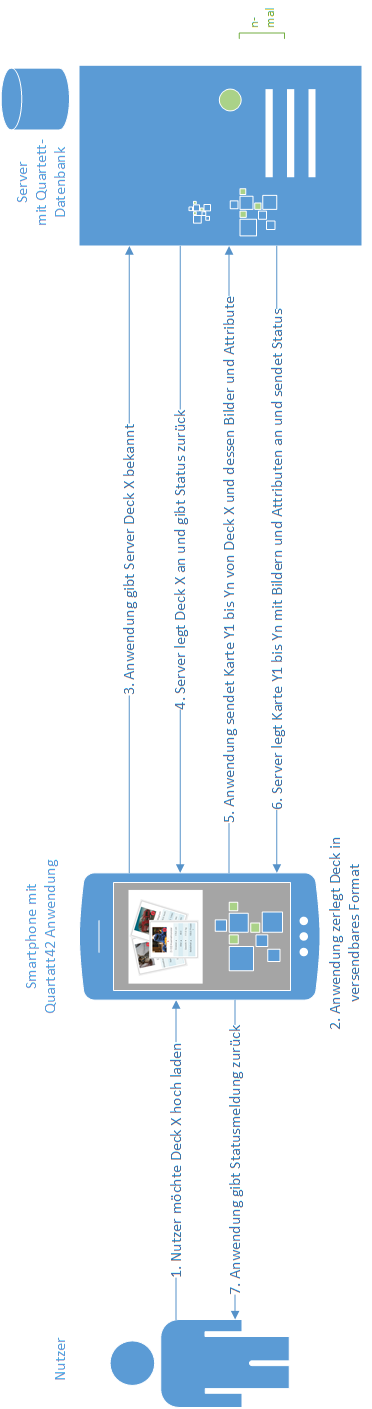
\includegraphics[width=.95\linewidth]{img/modelle/uploadmodell.png}
\end{minipage}%
\caption{Links: Downloadmodell, rechts: Uploadmodell }
\label{figure:implementierungdownundupload}
\end{figure}
%\newpage

% Abschnitt: Architektur
\section{Architektur}
\label{sec:implementierung:architektur}

\subsection{Datenmodell und -speicherung}
\label{sec:implementierung:architektur:datenmodell }

Für die Speicherung der Daten wollten wir ein möglichst einfaches, schnelles, aber auch platzsparendes Verfahren verwenden. Deswegen fiel die Wahl schnell auf eine Speicherung der Daten im JSON-Format. JSON bietet in diesem Fall einige Vorteile, wie zum Beispiel die kompakte Speicherung, eine einfache Handhabung, da die Daten in Javascript-Syntax gespeichert werden, und beliebige Erweiterbarkeit. Außerdem ermöglicht die Datenspeicherung im JSON-Format einige Vorteile, die durch klassische Datenbanken nicht gewährleistet sind, wie etwa die direkte Speicherung von Listen und Arrays. Aus diesem Grund entspricht unser Datenmodell nicht exakt den Diagrammen in Chen-Notation, ist aber an diese angelehnt.\\

\begin{figure}[htp]
	\centering
  	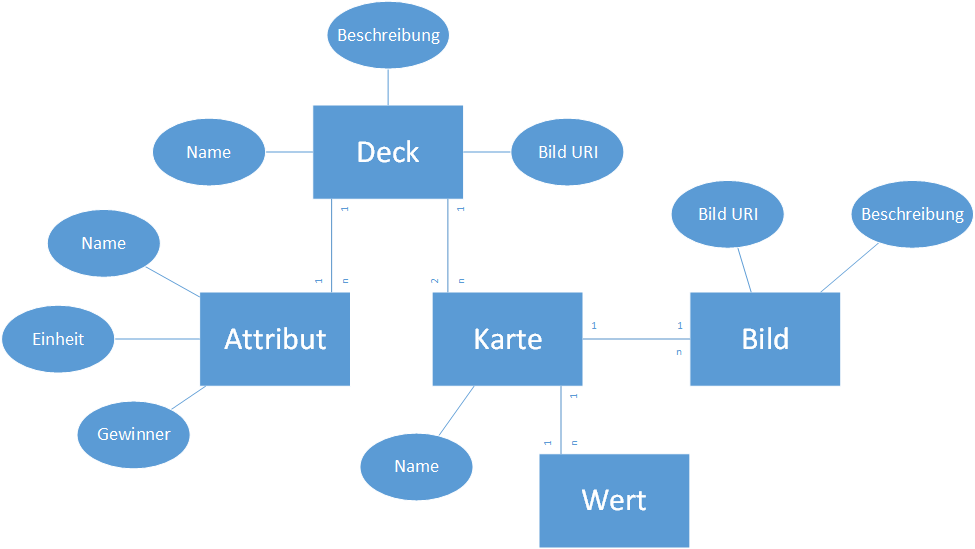
\includegraphics[width=\textwidth]{img/modelle/Datenmodell_aktualisiert.png}
	\caption{Datenmodell}
	\label{figure:implementierungdatenmodell}
\end{figure}

Gespeichert wird eine Liste von Decks. Jedes Deck enthält einen eindeutigen Namen und eine Beschreibung, sowie URI zu einem Bild. Außerdem enthält jedes Deck zwischen vier und zehn Attributen, welche einen für ein Deck eindeutigen Namen, eine Einheit und die Gewinnrichtung angeben. Dies erspart die Redundanz, die entstehen würde, wenn man diese Informationen bei jeder einzelnen Karte mit angeben müsste. Zu jedem Deck gehört eine Liste von mindestens zwei Karten. Diese haben jeweils neben einem für dieses Deck eindeutigen Namen ein oder mehrere Bilder, welches aus einer URI zu einem Bild und einer Beschreibung besteht. Außerdem enthält jede Karte gleich viele Werte, wie das Deck Attribute. Mit diesem einfachen Modell können sämtliche Daten gespeichert werden. Alle Einstellungen und laufenden Spiele werden direkt auf dem Smartphone über die SharedPreferences gespeichert, die von Android zur einfachen Speicherung kleinerer Datenmengen angeboten wird. Sämtliche Bilder werden direkt als Bitmap gespeichert und nur deren URI in den JSON-Daten verlinkt. Dabei werden die Bilder schon beim Speichern auf eine akzeptable Größe herunterskaliert.

\subsection{Klassen- und Activity-Architektur}
\label{sec:implementierung:architektur:klassenmodell }

\begin{figure}[htp]
	\centering
  	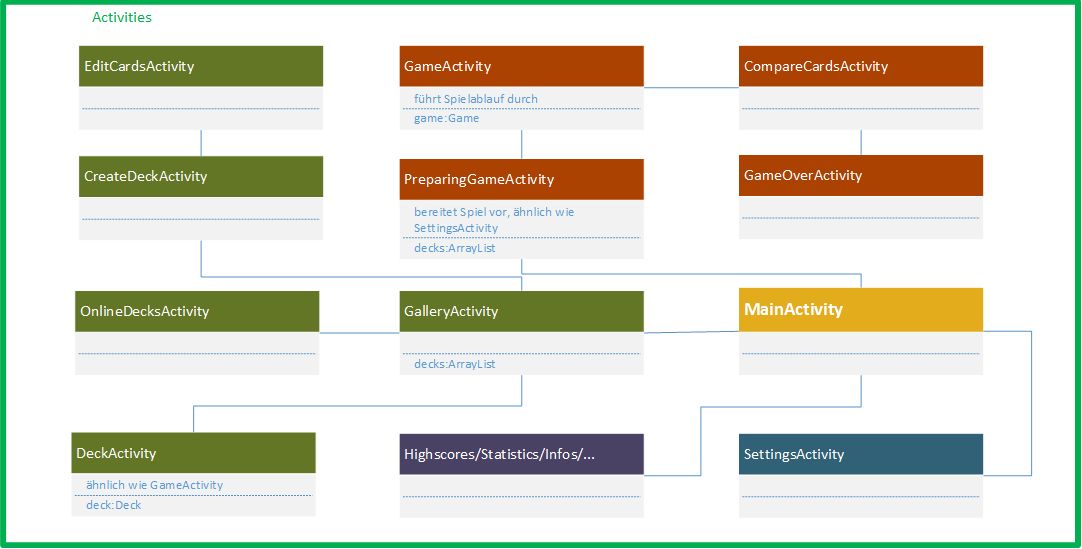
\includegraphics[width=\textwidth]{img/modelle/Klassenmodell_Activities.png}
	\caption{Activitymodell (vereinfacht)}
	\label{figure:implementierungactivitymodell}
\end{figure}

Die Architektur unserer Klassen entspricht mit kleinen Änderungen dem Datenmodell in Abbildung \ref{figure:implementierungdatenmodell}, weswegen wir es hier nicht noch einmal abbilden. Abbildung \ref{figure:implementierungactivitymodell} zeigt ein Modell der Activities unserer Anwendung. Dieses Modell beinhaltet alle Activities, welche durch eine Oberfläche für den Nutzer sichtbar und bedienbar sind. Es kann also gleichermaßen auch als GUI-Modell verstanden werden.

Zwischen den Activities gibt es natürlich noch weitere Verzweigungen. Zudem gibt es eine ganze Reihe von Hilfsklassen und -activities, die Hintergrundaufgaben durchführen, wie zum Beispiel das Handeln der Bilder, das Lesen und Schreiben der Daten im Speicher, die Kommunikation mit dem Server sowie das Durchführen der gesamten Spiellogik.

\subsection{Arbeitsaufteilung}
\label{sec:implementierung:architektur:arbeitsaufteilung }

Während der Implementation wurden die Aufgaben so aufgeteilt, dass jeder aus dem Team immer für eine bestimmte Aufgabe zuständig war und diese durch alle Schichten durch erledigen musste. Bei großen Aufgaben, wie dem Spielablauf, wurden die Aufgabe zudem in kleinere Schritte aufgeteilt. Da die App aus mehreren unabhängigen Bereichen besteht, konnten die Aufgaben gut eingeteilt werden, ohne dass es zu Behinderungen kommt. Wenn gerade keine Arbeit für eine Person angefallen war, beschäftigte diese sich mit Verbesserungen, Testen von Funktionen oder mit der Weiterentwicklung des Designs.

% Abschnitt: Schwierigkeiten während der Implementierung 
\section{Schwierigkeiten während der Implementierung}
\label{sec:implementierung:schwierigkeiten }	

In diesem Abschnitt möchten wir noch auf die größten Probleme eingehen, die wir während der Implementierung hatten, und wie wir diese gelöst haben. Generell muss man dazu sagen, dass es insgesamt doch zu deutlich weniger Problemen gekommen ist, als wir anfangs vermutet hatten. Und wenn Probleme aufkamen, hat man dank der ausführlichen Dokumentation und dank vielen Hilfen im Internet relativ schnell die Lösung dafür gefunden.

\begin{itemize} 
\item Ein großes Problem war der Umgang mit Bildern, da es dabei sehr viel zu beachten gibt. Wegen der unterschiedlichen Bildgrößen und -formate gab es Probleme, diese immer richtig und in der gleichen Größe darzustellen. Auch das  Speichern brachte verschiedene Probleme mit sich, bis wir den richtigen Speicherort und Speicherart gefunden haben, um nicht zu viel Platz zu verschwenden. Lösen konnten wir das Problem mit dem oben erwähnte Framework Picasso. Dieses nimmt einen sehr viel Arbeit im Umgang mit Bildern ab, wie das automatische Laden, Skalieren und Anzeigen von Bildern. Sehr lange Methoden konnten so durch einen ``Einzeiler'' ersetzt werden.
\item Ein weiteres Problem brachte der Umgang mit der Handygalerie, der Kamera und auch mit dem Abspielen von Sounds mit sich. An sich geht das alles sehr einfach mit Android. Die Probleme ergaben sich aber dann beim Testen auf den eigenen Handys und besonders am Emulator, da manche Funktionen hier nicht richtig funktionierten oder anders reagierten als erwartet. Erst nach reichlichem Ausprobieren funktionierte es auf allen Geräten.
\item An Stellen, an denen viele Zustände gespeichert werden müssen, wie beim Deckcreator, kam es zu Schwierigkeiten, diese zu speichern. Da der Nutzer jederzeit alle Werte ändern aber auch gleichzeitig zwischen allen Karten hin- und herwechseln können soll, führt das dazu, dass die Daten schlussendlich nach jeder einzelnen Interaktion im Deckcreator zwischengespeichert und überprüft werden müssen.
\item Auch der Datenaustausch zwischen den Activities hat uns Probleme bereitet, da diese außer bei primitiven Datentypen nicht trivial ist. Das lösten wir, indem wir versucht haben, den Datenaustausch zwischen den einzelnen Activities auf das Mindeste zu reduzieren und alle größeren Daten und Objekte aus dem Hintergrund zu laden.
\item Die wahrscheinlich meiste Zeit haben wir aber mit der GUI und dem Anordnen der Elemente auf der GUI-Ebene verbracht. Trotz den Möglichkeiten, den GUI-Builder zu benutzen, sah die GUI oft nicht aus wie gewünscht. Zudem gab es das Problem, dass eine GUI, die auf einem Smartphone gut aussah, auf einem anderen Smartphone ganz verschoben war oder Teile nicht sichtbar waren. Wenn man eine Anwendung für alle verschiedenen Bildschirmformate anpassen will, kann das viel Zeit und Nerven in Anspruch nehmen. Wir haben das ganze durch ein nicht all zu kompliziertes Design und durch viele wiederkehrende Designaspekte gelöst.
\end{itemize}